\chapter{O Método Simplex}

\section{Origem do Método Simplex}
O método simplex surgiu nos Estados Unidos e foi proposto pelo matemático George Dantzig. Quando trabalhava no Pentágono recebeu dos seus colegas o desafio de tentar mecanizar o processo de planejamento. No ano de 1947 Dantzig propôs o método simplex que tornou possível a solução de problemas de otimização de vários tipos, como transporte, produção, alocação de recursos e problemas de escalonamento \cite{OrigemSimplex}.

\section{Descrição do Método}
\subsection{Princípio Básico do Método}
A idéia do método simplex consiste em resolver repetidas vezes um sistema de equações lineares, e assim obter uma sucessão de soluções até encontrar a solução ótima. Ou seja, é um processo onde nos movemos de uma solução viável para outra sempre melhor ou pelo menos não pior.

Um problema de programação linear é sempre constituído de uma função objetivo e várias restrições. Geometricamente, essas restrições resultam em uma forma geométrica, chamada hiperplano, no espaço n-dimensional sendo n o número de variáveis no modelo. E cada vértice desse hiperplano é considerado uma solução viável, como ilustra o exemplo abaixo.
\begin{center}
	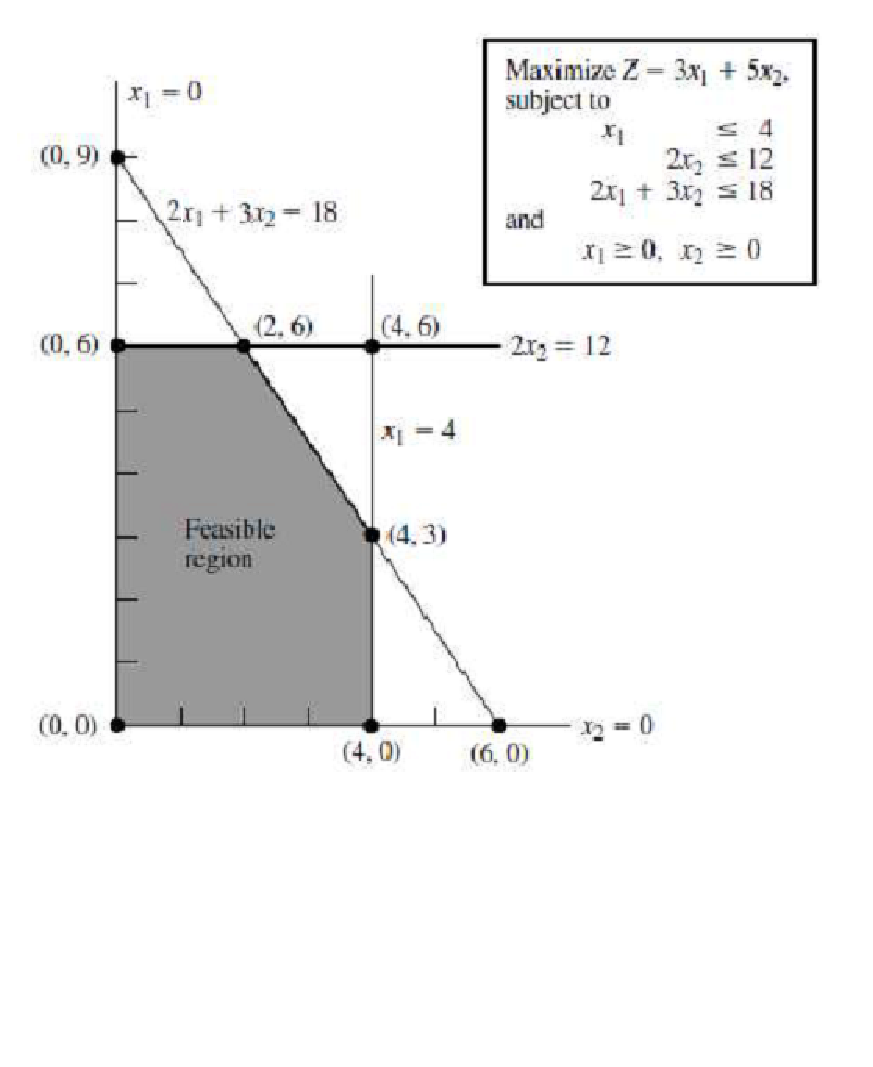
\includegraphics[scale=0.5]{graficos/Simplex_grafico_completo}
	\captionof{figure}{Um modelo de programação linear e a sua respectiva representação gráfica}
	\cite{Hillier}
\end{center}

Na Figura 1 apresenta-se um exemplo de um problema de programação linear e sua representação geométrica. Nesse exemplo, de acordo com a representação geométrica do modelo, existem cinco possíveis soluções: x1=0 e  x2=0; x1=0 e  x2=6; x1=2 e  x2=6; x1=4 e  x2=3; x1=4 e x2=0. Como o objetivo é maximizar, concluímos que a melhor solução é x1=2 e  x2=6, em que z =36. No método Simplex a cada iteração, antes da solução ótima ser obtida, é encontrada uma dessas possíveis soluções que se localizam nos vértices do gráfico.

\subsection{Descrição do Método Simplex Revisado}
O método simplex revisado surgiu como uma solução para evitar cálculos desnecessários. Esse método foi projetado para problemas a serem solucionados computacionalmente.

No simplex revisado, são armazenados na memória volátil apenas os dados realmente necessários. Além disso, os cálculos são realizados apenas sobre a coluna que é utilizada na iteração, o que evita cálculos com matrizes que poderia acarretar uma imprecisão nos resultados.

Esse método mantém a característica do simplex, que é a troca entre a variável que entra na base e a que sai, além de também exigir certo esforço computacional. Porém sua grande vantagem é a economia de tempo e espaço, que garantida pelo modo como é desenvolvida a solução. 

Nesta seção descreve-se os passos do algoritmo simplex revisado. O problema considerado é de maximização. A distinção entre matrizes, vetores e escalares foi feita da seguinte forma: letra maiúscula e negrito para matriz (\textbf{MATRIZ}); letra minúscula e negrito para vetor (\textbf{vetor}); letra em itálico para escalar (\textit{escalar}).

Considere o seguinte problema de programação linear:

$\\
Maximizar\ \mathbf{cx} \\
Sujeito\ a \\
\mathbf{Ax} \leq \mathbf{b} \\
\mathbf{x} \geq0$

O vetor $\mathbf{c}$, de coeficientes na função objetivo, é dividido duas componentes: $\mathbf{c{_B}}$ e $\mathbf{c{_N}}$, coeficientes das variáveis básicas e não-básicas, respectivamente. Por analogia, o vetor $\mathbf{x}$, de incógnitas do problema, é subdividido em $\mathbf{x{_B}}$ e $\mathbf{x{_N}}$.  A matriz $\mathbf{A}$, de coeficientes das restrições, é dividida em duas submatrizes: $\mathbf{B}$ e $\mathbf{N}$, coeficientes das variáveis básicas e não-básicas, respectivamente. Os passos do algoritmo são os seguintes.

Passo 1: Calcular o valor das variáveis básicas: $\mathbf{x_{b}}\ =\ \mathbf{B^{-1}b}\geq0$

Passo 2: Calcular o vetor multiplicador: $\mathbf{\lambda} \ =\ \mathbf{c{_B}B^{-1}}$

Passo 3: Escolher a variável que entra na base. Para isso, calcula-se: $\mathbf{p}\ =\ \mathbf{c{_N}}-\mathbf{\lambda N}$

Se $\mathbf{p}\ =\ (\mathbf{c{_N}}-\mathbf{\lambda N})\leq 0$ PARAR. A solução $\mathbf{x{_B}}$ já é a solução ótima. Caso contrário, escolher uma coluna de $\mathbf{N}$, coluna $\mathbf{a{_k}}$, tal que $\mathit{p{_k}}\ =\ \mathit{c{_nk}}-\mathbf{\lambda a{_k}}> 0$

Um critério frequente é escolher a coluna $\mathbf{a{_k}}$ que resulte no maior valor de $\mathit{p{_k}}$.

Então, assumindo $\mathit{e} = \mathit{k}$, $\mathit{k}$ representa o índice da coluna, $\mathbf{a{_k}}$ representa a coluna de $\mathbf{A}$ candidata a entrar na base. 

Passo 4: Determinar a variável que sai da base. Para isso, calcula-se: $\mathbf{y}=\mathbf{B^{-1}a{_k}}$

Se $\forall i\mathit{\frac{b{_i}}{y{_i}}}\leq 0$ PARAR A solução é não-limitada. Caso contrário, calcular:
$\forall i\ \underset{\underset{y{_i}>0}{1\leq i\leq m}}{Min}\begin{Bmatrix}
\mathit{\frac{b{_i}}{y{_i}}}
\end{Bmatrix}$ e guardar o índice correspondente a $s = i$. A variável $(x{_b}){_s}$ sai da base.

Passo 5: Criar a matriz $\mathbf{E}$.
$\mathbf{E}=(\mathbf{e{_1}},\mathbf{e{_2}},...,\mathbf{e{_s-1}},\mathbf{\gamma} , \mathbf{e{_s+1}},...,\mathbf{e{_m}})$

Onde, cada coluna da matriz é um vetor unitário com exceção da coluna $\mathit{s}$, que corresponde ao vetor $\mathbf{\gamma}$, calculado da seguinte maneira:
$\mathbf{\gamma^{t}}=\left( \mathit{\frac{-\alpha {_{1,e}}}{\alpha {_{s,e}}}}\ \mathit{\frac{-\alpha {_{2,e}}}{\alpha {_{s,e}}}}\ ...\ \mathit{\frac{-\alpha {_{s-1,e}}}{\alpha {_{s,e}}}}\ \mathit{\frac{1}{\alpha {_{s,e}}}\ \frac{-\alpha {_{s+1,e}}}{\alpha {_{s,e}}}}\ ...\ \mathit{\frac{-\alpha {_{m,e}}}{\alpha {_{s,e}}}} \right )$

Onde $\mathit{\alpha{_ie}}$ são os elementos vetor do $\mathbf{y}$.

Passo 6: Calcular nova matriz $\mathbf{B^{-1}}$: $\mathbf{B^{-1}} = \mathbf{EB^{-1}}$

Passo 7: Atualizar os vetores $\mathbf{c{_B}}$ e $\mathbf{x{_B}}$.
